% This is samplepaper.tex, a sample chapter demonstrating the
% LLNCS macro package for Springer Computer Science proceedings;
% Version 2.20 of 2017/10/04
%
\documentclass[runningheads]{llncs}
%
\usepackage{graphicx}
\usepackage{listings}
\usepackage{xcolor}
\usepackage{multicol}
\usepackage{amsmath}

% Define settings for SPARQL code highlighting
\lstdefinelanguage{SPARQL}{
  morekeywords={PREFIX, SELECT, WHERE, FILTER, OPTIONAL, UNION},
  sensitive=true,
  morecomment=[l]{\#},
  morestring=[b][\color{blue}]\",
}
\lstset{
  language=SPARQL,
  basicstyle=\tiny\ttfamily,
  keywordstyle=\color{purple},
  commentstyle=\color{gray},
  stringstyle=\color{blue},
  showstringspaces=false,
  breaklines=true,
  tabsize=2,
}

% Used for displaying a sample figure. If possible, figure files should
% be included in EPS format.
%
% If you use the hyperref package, please uncomment the following line
% to display URLs in blue roman font according to Springer's eBook style:
% \renewcommand\UrlFont{\color{blue}\rmfamily}

\newcommand{\todo}[1]{\textit{\textcolor{magenta}{Todo: #1}}}

\begin{document}
%
\title{Near Identity Relationships}
%\title{Abstracting Entity Matching for Analysing and Explaining Identity and Difference Decision and Indecision}
%
%\titlerunning{Abbreviated paper title}
% If the paper title is too long for the running head, you can set
% an abbreviated paper title here
%
% \author{First Author\inst{1}\orcidID{0000-1111-2222-3333} \and
% Second Author\inst{2,3}\orcidID{1111-2222-3333-4444} \and
% Third Author\inst{3}\orcidID{2222--3333-4444-5555}}
% %
% \authorrunning{F. Author et al.}
% % First names are abbreviated in the running head.
% % If there are more than two authors, 'et al.' is used.
% %
% \institute{Princeton University, Princeton NJ 08544, USA \and
% Springer Heidelberg, Tiergartenstr. 17, 69121 Heidelberg, Germany
% \email{lncs@springer.com}\\
% \url{http://www.springer.com/gp/computer-science/lncs} \and
% ABC Institute, Rupert-Karls-University Heidelberg, Heidelberg, Germany\\
% \email{\{abc,lncs\}@uni-heidelberg.de}}
%
\maketitle              % typeset the header of the contribution
%
%\begin{abstract}
%The abstract should briefly summarize the contents of the paper in
%15--250 words.

%\keywords{First keyword  \and Second keyword \and Another keyword.}
%\end{abstract}
%
%
%





\subsection{Near identity relationship}
In order to evaluate if entity matching contexts can help to identify pairs of entities engaged in a near identity relationship, we imagined the following scenario: In a first step a corpus of pairs of entities engaged in a near identity relationship is prepared by an expert. The near identity relationships represented by this corpus relate to a concept present in the world. It can be, for example the work of a writer or a film director. In a second step we compute all entity matching contexts for the pairs of the corpus. Given that there is an order of relation between contexts, we would like to know if keeping only the most representative properties of each context $\varepsilon$, $\Delta$ and $\Omega$ constitutes a reliable representation of the near identity relationship represented by this corpus.

In other words, the aim of this use case is to determine whether there are one or few representatives derived entity matching context \textit{patterns} that summarise the near-identity relationships. 
If so, it means that near identity relationships are detectable by the entity matching process through the entity matching contexts and patterns.
Otherwise it means that despite the corpus provided we are not able to summarise the near identity relationship to few patterns. 


In order to make this determination we need to: (i) build a corpus  that represents near-identity relationships, (ii) design a procedure that derive pattern(s) from a collection of entity matching contexts, (iii) compute EMCs  from the corpus build in (i) and discover pattern(s) with the procedure designed in (ii).
Finally (iv) we have to evaluate if pattern(s) is (are) representative of the corpus we have built up.
To do this we simply compute the support of pattern(s) on the collection of EMCs computed in (iii). 
    
The subsection is organised as follows. 
We first describe the building of 5 corpora.
We then briefly explain the pattern derivation procedure.
This procedure have been applied on the 5 corpora and  
we present patterns obtained. 
We have finally evaluated the representativeness of these patterns.

\subsubsection{Corpora construction}
We have built 5 corpora representing 2 different categories of near entity relationship. (i) relations that describe a more general concept than the one encoded in knowledge graphs (the concept of a literary or cinematographic work versus the concept of a book or film) and 
(ii) relationships that describe much more tenuous links between entities, entities linked together by their country.  
What motivated the construction of the second category was the construction of entity spaces as described by [Van Erp et \textit{al.} Toward Entity Spaces] , where the label Germany appears in three different contexts: the context of the meat industry, the context of the German population and the context of the German Davis Cup team. 
The table 1 presents for each corpus the type of entities used to build the pair, the property used to link these entities, and the number of author, director or countries present in each corpus. 
 
\begin{table}[]
    \centering
    \begin{tabular}{lcccc}
    \hline
    Corpus name & Entity 1 type & Entity 2 type & Link done on property & Nb   \\
    \hline
    &&&& \\
      \textbf{Literary Work}: books written  & & & & \\
      by the same author  & DBpedia Book & YAGO Book & author (created-inv) & 4928 authors\\
      & & & & \\
      \hline
      &&&& \\
      \textbf{Film Work}: films made  & & & & \\ 
      by the same director & DBpedia Film & YAGO Film & director (created-inv) & 8500 film directors \\
      & & & & \\
    \hline
    \hline
    &&&& \\
     \textbf{Book University}: books and & & & & \\ 
     universities located in the & & & & \\
     same country & DBpedia Book & DBpedia University & islocatedin & 126 countries \\
     & & & & \\
     \hline
     &&&& \\
     \textbf{Book Mountain}: books and &&&& \\
     mountains located in the &&&& \\
     same country& DBpedia Book & DBpedia Mountain & islocatedin & 143 countries\\
     & & & & \\
     \hline
     &&&& \\
     \textbf{Mountain University}: &&&& \\
     mountains and universities  &&&& \\
     located in the same country& DBpedia Mountain & DBedia University & islocatedin & 598 countries \\
     & & & & \\
     \hline
    \end{tabular}
    \caption{Description of the 5 corpora.}
    \label{tab:corpus-construction}
\end{table}

\subsubsection{Pattern Detection Procedure}
To explicit patterns detection we present here a toy example. The table 2 presents 3 EMCs computed from pairs of books of Agatha Christie. The pairs share the same author in each case, but titles (label) differs and the number of pages or the isbn number are missing.  The last line of the table represents the pattern derived from these 3 relationships. Notice that in this toy example, all the EMCs matches with the pattern detected, we obtain a coverage of 100\%. 


\subsubsection{Pattern Discovery and Evaluation}
In the same idea we performed pattern discovery (i) on the Literary Work and Film Work corpora and (ii) on the 3 corpora of books, mountains and universities from the same country. The first row of Table 3 shows that 90\% of the pairs from the literary works corpus are recognised by a single pattern $P1=\{created-inv\},\{skos:preflabel\},\{wascreatedonyear\}$. The second line shows that 2 patterns ($P2$ and $P3$) need to be combined for 90\% of the pairs in the cinematographic corpus to be recognised. The second part of Table 3 shows that 96\% of pairs from the book-mountain and book-university corpora are recognised by the same parttern. But it takes a combination of 4 patterns to recognise 98\% pairs of the mountain-university corpus.
It appears that, on the 5 corpora studied, it is possible to summarise near-identity relationships with few patterns. 

\begin{table}[]
    \centering
    \begin{tabular}{llll}
        \multicolumn{4}{l}{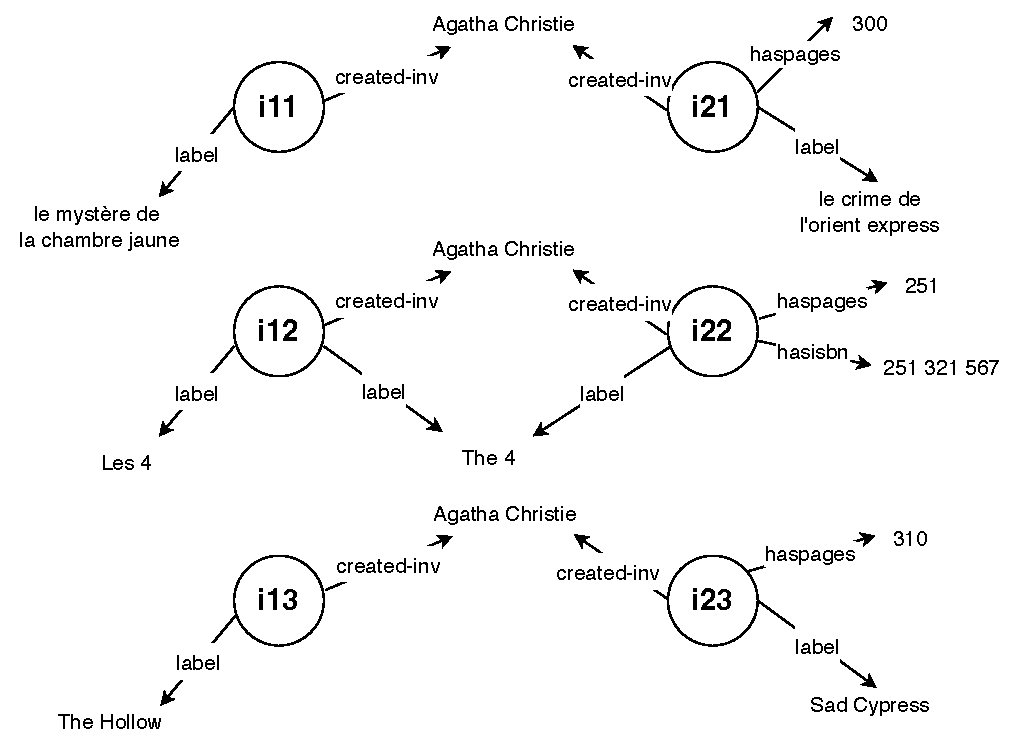
\includegraphics[scale=0.7]{./agatha.pdf}} \\
        %\hline
         i11,i21 & \{created-inv\}& \{label\}&\{haspages\} \\
         i12,i22 & \{created-inv,label\}&\{label\} &\{haspages,hasisbn\} \\
         i13,i23 & \{created-inv\}&\{label\}&\{has-pages\}\\
        \hline
        
        pattern & \{created-inv\}&\{label\}&\{has-pages\} \\
        
    \end{tabular}
    \caption{The example of pattern construction based on 3 EMCs.}
    \label{tab:pattern_example}
\end{table}

\begin{table}[]
    \centering
    \begin{tabular}{l|l|c|c|c}
        \hline
         corpus & pattern $\varepsilon\Delta\Omega$ & nb match & total nb EMCs & coverage   \\
         \hline
       literary work  & & & & \\
         & P1=\{created-inv\},\{skos:preflabel\},\{wascreatedonyear\}& & & \\
       \hline  
       & P1 & 148281 & 165508 & 0.90\\
       \hline
       film work & & & & \\  
       & P2=\{directed-inv\}\{skos:preflabel\},\{wascreatedonyear\} & & & \\
       & P3=\{directed-inv\}\{skos:preflabel\},\{islocatedin\} & & & \\
       \hline
        & P2 $\cup$ P3 & 606529 & 674952 & 0.90\\
       %\hline
       \hline
       \hline
       book mountain & & & & \\  
       & P4=\{islocatedin\},\{skos:preflabel\}, \{created-inv\}& & & \\
       \hline
       & P4 & 15320925 & 15993180 & 0.96\\
       \hline
       book university & & & &  \\
       & P5=\{islocatedin\},\{skos:preflabel\},\{created-inv\}& & & \\
       \hline
       & P5 & 15320840 & 15993082 & 0.96 \\
       \hline
       mountain university  & & & & \\
       & P6=\{islocatedin\},\{islocatedin\},\{haslatitude\}, \{haslongitude\}& & & \\
       &P7=\{islocatedin\},\{islocatedin\},\{graduatedfrom-inv\}& & & \\
       &P8=\{islocatedin\}\{islocatedin\},\{\}& & & \\
       &P9=\{islocatedin\}\{islocatedin\},\{hasmotto\}& & & \\
       \hline
       &P6 $\cup$ P7 $\cup$ P8 $\cup$ P9 & 4708646 & 4795678& 0.98\\
       \hline
    \end{tabular}
    \caption{Patterns detection on corpora.The coverage is computed as follows: $\frac{nb\_EMCs\_that\_matches\_pattern}{nb\_total\_ EMCs}$}
    \label{tab:pattern_detection}
\end{table}

\subsection{Code}
Corpora construction, pattern detection and representativeness evaluation are available in the following scripts:
\begin{itemize}
	\item iswc2024/pattern/author\_work\_pattern.py for the corpus author work
	\item iswc2024/pattern/director\_work\_pattern.py for the corpus cinematographic work
	\item iswc2024/pattern/country\_work\_pattern.py for the 3 corpora of entities linked by their countries 
\end{itemize}

\end{document}
